\subsection{Descripción del dataset}

Los datasets que se van a usar han sido recopilados por Luis Castillo Vidal y corresponden a la actividad de sus alumnos en la asignatura \href{https://www.ugr.es/estudiantes/grados/grado-ingenieria-informatica/desarrollo-basado-agentes-ing-software}{\color{blue}{Desarrollo Basado en Agentes}}.

El primer dataset, tras haber sido filtrados los registros erróneos, consta de 47828 filas correspondientes a los diferentes acciones de unos drones en una serie de mundos virtuales. En cada registro se detallan los siguientes atributos:
\begin{itemize}
\item \emph{year}: identifica el curso académico en el que se realizó dicha acción.
\item \emph{group}: grupo de prácticas que ha prograda al dron que acomete la acción.
\item \emph{date}: fecha en la que se lleva a cabo la acción.
\item \emph{map}: mundo virtual en el que se ha realizado la acción.
\item \emph{action}: indica el tipo de acción realizada.
\end{itemize}
% Dimesiones: 47828 registros, 5 columnas por registro.

En la Tabla \ref{table:1} se presentan los primeros seis registros del dataset. Además, en la Tabla \ref{table:2} puede apreciarse un resumen de los datos que tenemos.

% Muestra del dataset 1
% latex table generated in R 4.2.2 by xtable 1.8-4 package
% Wed Feb  1 15:07:17 2023
\begin{table}[ht]
\centering
\begin{tabular}{rlllll}
  \hline
 & year & group & date & map & action \\ 
  \hline
1 & 1516 & Achernar & 17/10/2015 19:41:45 & 0 & 0 \\ 
  2 & 1516 & Bellatrix & 17/10/2015 19:41:45 & 0 & 0 \\ 
  3 & 1516 & Cerastes & 17/10/2015 19:41:45 & 0 & 0 \\ 
  4 & 1516 & Denebola & 17/10/2015 19:41:45 & 0 & 0 \\ 
  5 & 1516 & Elnath & 17/10/2015 19:41:45 & 0 & 0 \\ 
  6 & 1516 & Furud & 17/10/2015 19:41:45 & 0 & 0 \\ 
   \hline
\end{tabular}
\caption{Muestra del primer dataset}
\label{table:1}
\end{table}

% Resumen del dataset que tenemos:
% latex table generated in R 4.2.2 by xtable 1.8-4 package
% Wed Feb  1 15:08:53 2023
\begin{table}[ht]
\centering
\begin{tabular}{lllll}
  \hline
     year &    group &     date &      map &     action \\ 
  \hline
Min.   :1516   & Length:47828       & Length:47828       & Min.   :0.000   & Min.   :0.000   \\ 
  1st Qu.:1516   & Class :character   & Class :character   & 1st Qu.:1.000   & 1st Qu.:1.000   \\ 
  Median :1617   & Mode  :character   & Mode  :character   & Median :3.000   & Median :2.000   \\ 
  Mean   :1700   &  &  & Mean   :3.834   & Mean   :2.325   \\ 
  3rd Qu.:1920   &  &  & 3rd Qu.:6.000   & 3rd Qu.:3.000   \\ 
  Max.   :1920   &  &  & Max.   :9.000   & Max.   :5.000   \\ 
   \hline
\end{tabular}
\caption{Resumen del primer dataset que tenemos}
\label{table:2}
\end{table}

La Figuras \ref{fig:boxplotmap} y \ref{fig:boxplotaction} muestran, respectivamente, los gráficos de caja y bigotes de las variables \emph{map} y \emph{action}.

\begin{figure}[!tbp]
  \begin{subfigure}[b]{0.49\textwidth}
    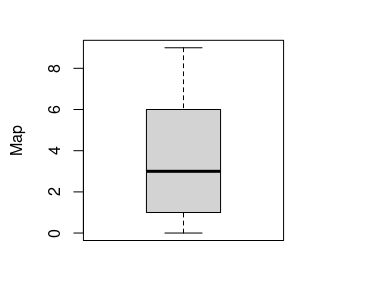
\includegraphics[width=\textwidth, height=\textwidth]{imagenes/Rplot02.png}
    \caption{Gráfico de caja y bigotes de la variable \emph{map}}
    \label{fig:boxplotmap}
  \end{subfigure}
  \hfill
  \begin{subfigure}[b]{0.49\textwidth}
    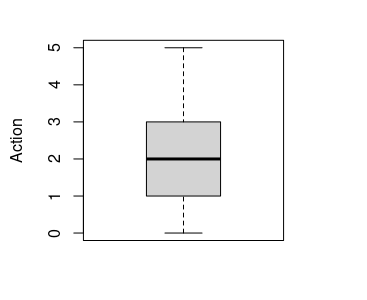
\includegraphics[width=\textwidth, height=\textwidth]{imagenes/Rplot04.png}
    \caption{Gráfico de caja y bigotes de la variable \emph{action}}
    \label{fig:boxplotaction}
  \end{subfigure}
  \caption{Diagramas de caja y bigotes de las variables \emph{map} y \emph{action}}
\end{figure}

Además, podemos ver la distribución de los diferentes niveles del factor \emph{map} y de los diferentes niveles del factor \emph{action} en las Figuras \ref{fig:yearmap} y \ref{fig:yearaction}.

\begin{figure}[!tbp]
  \begin{subfigure}[b]{0.49\textwidth}
    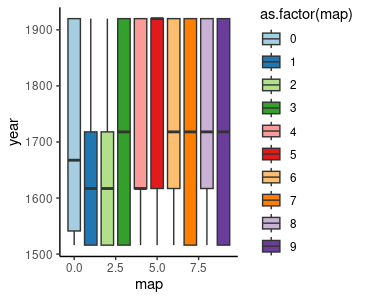
\includegraphics[width=\textwidth, height=\textwidth]{imagenes/Rplot.png}
    \caption{Distribución de los diferentes niveles del factor \emph{map}}
    \label{fig:yearmap}
  \end{subfigure}
  \hfill
  \begin{subfigure}[b]{0.49\textwidth}
    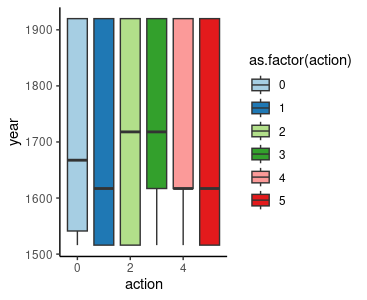
\includegraphics[width=\textwidth, height=\textwidth]{imagenes/Rplot01.png}
    \caption{Distribución de los diferentes niveles del factor \emph{action}}
    \label{fig:yearaction}
  \end{subfigure}
  \caption{Distribuciones para diferentes niveles de los factores}
\end{figure}

Por último, también podemos ver la distribución de las variables \emph{map} y \emph{action} en función del año (variable \emph{year}) en las Figuras \ref{fig:mapyear} y \ref{fig:actionyear}.

\begin{figure}[!tbp]
  \begin{subfigure}[b]{0.49\textwidth}
    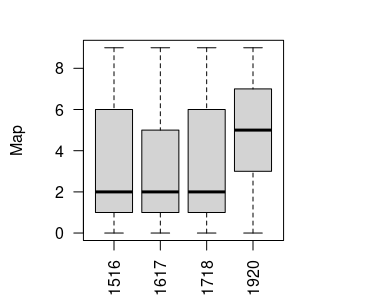
\includegraphics[width=\textwidth, height=\textwidth]{imagenes/Rplot03.png}
    \caption{Distribución de la variable \emph{map} en función de \emph{year}}
    \label{fig:mapyear}
  \end{subfigure}
  \hfill
  \begin{subfigure}[b]{0.49\textwidth}
    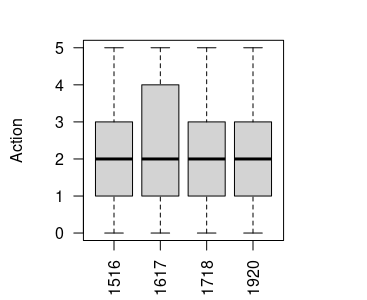
\includegraphics[width=\textwidth, height=\textwidth]{imagenes/Rplot05.png}
    \caption{Distribución de la variable \emph{action} en función de \emph{year}}
    \label{fig:actionyear}
  \end{subfigure}
  \caption{Distribuciones de las variables \emph{map} y \emph{action} dependiendo del valor de \emph{year}}
\end{figure}

El segundo dataset, tras haber sido eliminados algunas columnas que no eran interesantes para nuestro estudio, consta de 118 filas correspondientes a las diferentes calificaciones de los equipos en las dos prácticas realizadas en la asignatura \href{https://www.ugr.es/estudiantes/grados/grado-ingenieria-informatica/desarrollo-basado-agentes-ing-software}{\color{blue}{Desarrollo Basado en Agentes}}. En cada registro se detallan los siguientes atributos:
\begin{itemize}
\item \emph{Group}: grupo de prácticas que ha prograda al dron.
\item \emph{Team}: cadena de texto que identifica el curso académico en el que se realizó dicha acción, la práctica realizada y el grupo de prácticas conjuntamente.
\item \emph{Size}: tamaño del grupo de práctcas.
\item \emph{Year}: identifica el curso académico en el que se realizó dicha acción.
\item \emph{Grade}: calificación obtenida por el grupo de prácticas.
\end{itemize}
% Dimesiones: 118 registros, 5 columnas por registro.

En la Tabla \ref{table:6} se presentan los primeros seis registros del dataset. Además, en la Tabla \ref{table:7} puede apreciarse un resumen de los datos que tenemos.

% Muestra del dataset 2
% latex table generated in R 4.2.2 by xtable 1.8-4 package
% Sun Feb  5 13:27:02 2023
\begin{table}[ht]
\centering
\begin{tabular}{rlllll}
  \hline
 & Group & Team & Size & Year & Grade \\ 
  \hline
1 & G1 & DBA 1819 P3 GL & 4 & 1819 & 10,00 \\ 
  2 & G2 & DBA 1920 P3 GJ & 4 & 1920 & 4,01 \\ 
  3 & G3 & DBA 1819 P2 GH & 4 & 1819 & 7,96 \\ 
  4 & G4 & DBA 1920 P2 GE & 4 & 1920 & 8,95 \\ 
  5 & G5 & DBA 1920 P3 GK & 4 & 1920 & 4,51 \\ 
  6 & G6 & DBA 1415 P3 G6 & 6 & 1415 & 7,20 \\ 
   \hline
\end{tabular}
\caption{Muestra del segundo dataset}
\label{table:6}
\end{table}

% latex table generated in R 4.2.2 by xtable 1.8-4 package
% Sun Feb  5 13:31:46 2023
\begin{table}[ht]
\centering
\begin{tabular}{lllll}
  \hline
   Group &     Team &      Size &      Year &    Grade \\ 
  \hline
Length:118         & Length:118         & Min.   :3.000   & Min.   :1314   & Length:118         \\ 
  Class :character   & Class :character   & 1st Qu.:4.000   & 1st Qu.:1516   & Class :character   \\ 
  Mode  :character   & Mode  :character   & Median :5.000   & Median :1718   & Mode  :character   \\ 
   &  & Mean   :4.831   & Mean   :1662   &  \\ 
   &  & 3rd Qu.:6.000   & 3rd Qu.:1819   &  \\ 
   &  & Max.   :6.000   & Max.   :1920   &  \\ 
   \hline
\end{tabular}
\caption{Resumen del segundo dataset que tenemos}
\label{table:7}
\end{table}

\subsection{Introducción}

En este estudio inicial se desarrollará un modelo estadístico para determinar el efecto de los parámetros \emph{map} y \emph{action} (dos varibles explicativas) en la variable respuesta \emph{year}.

La relevancia de cada una de las variables en el modelo se determinará por el test \emph{two way ANOVA} con un $5\%$ de nivel de significancia y se empleará la técnica de los \emph{mínimos cuadrados} para estimar los coeficientes del modelo considerado.

\subsection{Two way ANOVA}

Un resumen de los resultados obtenidos al realizar el test two way ANOVA se muestra en la Tabla \ref{table:3}. Puede observarse que la variable \emph{map} es significante al nivel $0$, que la variable \emph{action} es significante al nivel $0.01$ y que la variable \emph{map:action} (el término de interacción) no es significante. Así pues, puede concluirse que el dataset es homógeneo, es decir, las combinaciones \emph{map:action} son estadísticamente iguales en todos los años considerados.

%Resumen two way ANOVA test:
% latex table generated in R 4.2.2 by xtable 1.8-4 package
% Wed Feb  1 15:19:36 2023
\begin{table}[ht]
\centering
\begin{tabular}{lrrrrr}
  \hline
 & Df & Sum Sq & Mean Sq & F value & Pr($>$F) \\ 
  \hline
map         & 1 & 62918413.58 & 62918413.58 & 2689.15 & 0.0000 \\ 
  action      & 1 & 101244.69 & 101244.69 & 4.33 & 0.0375 \\ 
  map:action  & 1 & 8797.03 & 8797.03 & 0.38 & 0.5398 \\ 
  Residuals   & 47824 & 1118946173.13 & 23397.17 &  &  \\ 
   \hline
\end{tabular}
\caption{Resultados del test two way ANOVA}
\label{table:3}
\end{table}

La notación escalar del modelo ajustado al aplicar el test tiene la siguiente estructura:

\begin{equation}
    y = \beta_0 + \beta_1 \cdot x_1 + \beta_2 \cdot x_2 + \beta_3 \cdot x_1 \cdot x_2 + \epsilon
\label{eq1}
\end{equation}

donde $\beta_0$ es el intercepto, $\beta_1$ y $\beta_2$ son los coeficientes de los efectos principales, $\beta_3$ es el coeficiente del término de interacción, $x_1$ y $x_2$ son los parámetros sometidos a investigación (en este caso, $x_1$ representa el parámetro mapa y $x_2$ representa la acción), $y$ representa el año y $\epsilon$ es el \emph{término error}.

La Tabla \ref{table:4} muestra los valores de los coeficientes de la fórmula que se han obtenido tras ajustar el modelo de regresión a los datos.

%Coeficientes del modelo:
% latex table generated in R 4.2.2 by xtable 1.8-4 package
% Wed Feb  1 15:20:53 2023
\begin{table}[ht]
\centering
\begin{tabular}{rr}
  \hline
 & x \\ 
  \hline
(Intercept) & 1655.03 \\ 
  map & 12.31 \\ 
  action & -1.51 \\ 
  map:action & 0.12 \\ 
   \hline
\end{tabular}
\caption{Coeficientes del modelo}
\label{table:4}
\end{table}

La Figura \ref{fig:interaccion} muestra la interacción entre los parámetros mapa y acción. Así pues, puede observarse que todas las líneras de la gráfica siguen más o menos el mismo patrón, lo que evidencia que no hay una gran interacción entre ambos.

\begin{figure}[h]
    \centering
    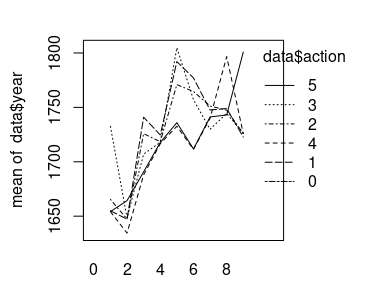
\includegraphics[width=0.60\textwidth]{imagenes/Rplot06.png}
    \caption{Interacción entre las variables \emph{map} y \emph{action}}
    \label{fig:interaccion}
\end{figure}

% Tukey multiple comparisons of means
% 95% family-wise confidence level
% Fit: aov(formula = year ~ map * action, data = data)
% $map

La Figura \ref{fig:suposiciones} muestra que no se violan las suposiciones que hemos realizado sobre el modelo. La media y la varianza de los residuos no parece que varíe respecto de los valores ajustados. Como consecuencia, conluiré que podemos suponer la homocedasticidad. Además, si nos fijamos en el \emph{Normal Q-Q plot}, puede observarse que los residuos son gaussianos.

\begin{figure}[h]
    \centering
    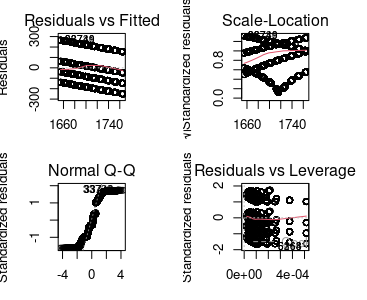
\includegraphics[width=0.60\textwidth]{imagenes/Rplot07.png}
    \caption{Gráficas diagnósticas del modelo ANOVA}
    \label{fig:suposiciones}
\end{figure}

\subsection{Segmentación de los datos}

Se ha realizado una segmentación de los registros del primer dataset en función de la calificación obtenida por los grupos que han realizado las acciones en los mapas.

Para ello, se ha sustituido la columna \emph{Team} del segundo dataset por el nombre del grupo en cada caso y se ha eliminado la columna \emph{Group}. Después de realizar este proceso el dataset tiene la forma que se muestra en la Tabla \ref{table:8}

% Segundo dataset tras cambiar el contenido de la columna Team
% latex table generated in R 4.2.2 by xtable 1.8-4 package
% Sun Feb  5 13:39:47 2023
\begin{table}[ht]
\centering
\begin{tabular}{rllll}
  \hline
 & group & size & year & grade \\ 
  \hline
1 & Lesath & 4 & 1819 & 10,00 \\ 
  2 & Jabbah & 4 & 1920 & 4,01 \\ 
  3 & Haldus & 4 & 1819 & 7,96 \\ 
  4 & Elnath & 4 & 1920 & 8,95 \\ 
  5 & Keid & 4 & 1920 & 4,51 \\ 
  6 & Furud & 6 & 1415 & 7,20 \\ 
   \hline
\end{tabular}
\caption{Dataset 2 tras ser preparado para hacer join}
\label{table:8}
\end{table}

A continuación, se transformarán los valores de la columna \emph{grade} a tipo \texttt{double} y se agruparán los datos de este dataset por grupo y año, calculando la calificación media de las prácticas para cada par grupo-año. El resultado de realizar esta operación puede apreciarse ne la Tabla \ref{table:9}.

% Agrupación del segundo dataset por grupo y año
% latex table generated in R 4.2.2 by xtable 1.8-4 package
% Sun Feb  5 13:46:44 2023
\begin{table}[ht]
\centering
\begin{tabular}{rllll}
  \hline
 & group & year & size & mean\_grade \\ 
  \hline
1 & Achernar & 1314 & 6 &  9.40 \\ 
  2 & Achernar & 1415 & 5 &  9.00 \\ 
  3 & Achernar & 1516 & 5 &  8.20 \\ 
  4 & Achernar & 1617 & 5 & 10.00 \\ 
  5 & Achernar & 1718 & 5 &  8.33 \\ 
  6 & Bellatrix & 1516 & 5 &  8.20 \\ 
   \hline
\end{tabular}
\caption{Dataset 2 tras agrupar por grupo y año}
\label{table:9}
\end{table}

Ahora, se juntan ambos datasets usando la función \texttt{inner\_join} por grupo y año. El resultado de esta operación puede observarse en la Tabla \ref{table:10}.

% inner_join de los dos datasets
% latex table generated in R 4.2.2 by xtable 1.8-4 package
% Sun Feb  5 13:50:57 2023
\begin{table}[ht]
\centering
\begin{tabular}{rlllllll}
  \hline
 & group & year & size & mean\_grade & date & map & action \\ 
  \hline
1 & Achernar & 1516 & 5 & 8.2 & 17/10/2015 19:41:45 & 0 & 0 \\ 
  2 & Achernar & 1516 & 5 & 8.2 & 22/10/2015 17:29:21 & 1 & 1 \\ 
  3 & Achernar & 1516 & 5 & 8.2 & 22/10/2015 17:29:22 & 1 & 2 \\ 
  4 & Achernar & 1516 & 5 & 8.2 & 22/10/2015 17:29:39 & 1 & 3 \\ 
  5 & Achernar & 1516 & 5 & 8.2 & 22/10/2015 17:34:09 & 1 & 1 \\ 
  6 & Achernar & 1516 & 5 & 8.2 & 22/10/2015 17:34:10 & 1 & 2 \\ 
   \hline
\end{tabular}
\caption{Unión de ambos datasets}
\label{table:10}
\end{table}

Por último, se separarán los datos de esta última tabla en función de las calificaciones obtenidas por los diferentes grupos:
\begin{itemize}
	\item \textbf{Suspenso:} calificación mayor o igual que $0$ y menor que $5$.
	\item \textbf{Aprobado:} calificación mayor o igual que $5$ y menor que $7$.
	\item \textbf{Notable:} calificación mayor o igual que $7$ y menor que $9$.
	\item \textbf{Sobresaliente:} calificación mayor o igual qye $9$ y menor que $10$.
	\item \textbf{Matrícula de Honor:} calificación igual a $10$.
\end{itemize}

Una muestra de los datasets generados tras la segmentación puede apreciarse en las tablas \ref{table:11}, \ref{table:12}, \ref{table:13}, \ref{table:14} y \ref{table:15}.

% latex table generated in R 4.2.2 by xtable 1.8-4 package
% Sun Feb  5 18:45:16 2023
\begin{table}[ht]
\centering
\begin{tabular}{rlllllll}
  \hline
 & group & year & size & mean\_grade & date & map & action \\ 
  \hline
1 & Girtab & 1617 & 6 & 4.67 & 15/11/2016 7:31:31  & 1 & 1 \\ 
  2 & Girtab & 1617 & 6 & 4.67 & 15/11/2016 7:31:53  & 1 & 1 \\ 
  3 & Girtab & 1617 & 6 & 4.67 & 15/11/2016 12:50:03 & 1 & 1 \\ 
  4 & Girtab & 1617 & 6 & 4.67 & 15/11/2016 12:50:28 & 1 & 1 \\ 
  5 & Girtab & 1617 & 6 & 4.67 & 15/11/2016 13:27:27 & 1 & 1 \\ 
  6 & Girtab & 1617 & 6 & 4.67 & 15/11/2016 13:27:58 & 1 & 1 \\ 
   \hline
\end{tabular}
\caption{Muestra del dataset de los grupos \textbf{suspensos}. Consta de $2397$ registros con $7$ campos cada uno.}
\label{table:11}
\end{table}

% latex table generated in R 4.2.2 by xtable 1.8-4 package
% Sun Feb  5 18:47:50 2023
\begin{table}[ht]
\centering
\begin{tabular}{rlllllll}
  \hline
 & group & year & size & mean\_grade & date & map & action \\ 
  \hline
1 & Bellatrix & 1920 & 4 & 6.835 & 05/11/2019 10:24:51 & 1 & 1 \\ 
  2 & Bellatrix & 1920 & 4 & 6.835 & 05/11/2019 10:24:51 & 1 & 2 \\ 
  3 & Bellatrix & 1920 & 4 & 6.835 & 05/11/2019 10:25:04 & 1 & 1 \\ 
  4 & Bellatrix & 1920 & 4 & 6.835 & 05/11/2019 10:25:26 & 1 & 2 \\ 
  5 & Bellatrix & 1920 & 4 & 6.835 & 05/11/2019 10:25:39 & 1 & 1 \\ 
  6 & Bellatrix & 1920 & 4 & 6.835 & 05/11/2019 10:25:45 & 1 & 2 \\ 
   \hline
\end{tabular}
\caption{Muestra del dataset de los grupos \textbf{aprobados}. Consta de $7053$ registros con $7$ campos cada uno.}
\label{table:12}
\end{table}

% latex table generated in R 4.2.2 by xtable 1.8-4 package
% Sun Feb  5 18:50:12 2023
\begin{table}[ht]
\centering
\begin{tabular}{rlllllll}
  \hline
 & group & year & size & mean\_grade & date & map & action \\ 
  \hline
1 & Achernar & 1516 & 5 & 8.2 & 17/10/2015 19:41:45 & 0 & 0 \\ 
  2 & Achernar & 1516 & 5 & 8.2 & 22/10/2015 17:29:21 & 1 & 1 \\ 
  3 & Achernar & 1516 & 5 & 8.2 & 22/10/2015 17:29:22 & 1 & 2 \\ 
  4 & Achernar & 1516 & 5 & 8.2 & 22/10/2015 17:29:39 & 1 & 3 \\ 
  5 & Achernar & 1516 & 5 & 8.2 & 22/10/2015 17:34:09 & 1 & 1 \\ 
  6 & Achernar & 1516 & 5 & 8.2 & 22/10/2015 17:34:10 & 1 & 2 \\ 
   \hline
\end{tabular}
\caption{Muestra del dataset de los grupos con \textbf{notable}. Consta de $18840$ registros con $7$ campos cada uno.}
\label{table:13}
\end{table}

% latex table generated in R 4.2.2 by xtable 1.8-4 package
% Sun Feb  5 18:51:55 2023
\begin{table}[ht]
\centering
\begin{tabular}{rlllllll}
  \hline
 & group & year & size & mean\_grade & date & map & action \\ 
  \hline
1 & Bellatrix & 1617 & 5 & 9.72 & 07/11/2016 11:13:31 & 1 & 1 \\ 
  2 & Bellatrix & 1617 & 5 & 9.72 & 07/11/2016 11:36:59 & 1 & 1 \\ 
  3 & Bellatrix & 1617 & 5 & 9.72 & 07/11/2016 11:41:07 & 1 & 1 \\ 
  4 & Bellatrix & 1617 & 5 & 9.72 & 07/11/2016 11:42:22 & 1 & 1 \\ 
  5 & Bellatrix & 1617 & 5 & 9.72 & 07/11/2016 11:45:37 & 1 & 1 \\ 
  6 & Bellatrix & 1617 & 5 & 9.72 & 07/11/2016 11:49:23 & 1 & 1 \\ 
   \hline
\end{tabular}
\caption{Muestra del dataset de los grupos con \textbf{sobresaliente}. Consta de $17891$ registros con $7$ campos cada uno.}
\label{table:14}
\end{table}

% latex table generated in R 4.2.2 by xtable 1.8-4 package
% Sun Feb  5 18:53:13 2023
\begin{table}[ht]
\centering
\begin{tabular}{rlllllll}
  \hline
 & group & year & size & mean\_grade & date & map & action \\ 
  \hline
1 & Achernar & 1617 & 5 & 10 & 09/11/2016 21:23:22 & 1 & 1 \\ 
  2 & Achernar & 1617 & 5 & 10 & 09/11/2016 21:25:11 & 1 & 1 \\ 
  3 & Achernar & 1617 & 5 & 10 & 10/11/2016 0:21:37  & 1 & 1 \\ 
  4 & Achernar & 1617 & 5 & 10 & 10/11/2016 0:22:50  & 1 & 1 \\ 
  5 & Achernar & 1617 & 5 & 10 & 10/11/2016 0:23:12  & 1 & 1 \\ 
  6 & Achernar & 1617 & 5 & 10 & 10/11/2016 0:25:53  & 1 & 1 \\ 
   \hline
\end{tabular}
\caption{Muestra del dataset de los grupos con \textbf{matrícula de honor}. Consta de $1646$ registros con $7$ campos cada uno.}
\label{table:15}
\end{table}